\section{Previous Work} \label{sec:previous_work}
A first version of PowerPedia already exists. It was implemented as part of Adrian Merkle's Master thesis~\cite{merklepp}. This prototype was realized as an extension to the eMeter system, which is described further thereafter.
In order to demonstrate the functionality of Powerpedia, Merkle also implemented an Android eMeter application based on the already existing iPhone application. This mobile phone application serves as a user interface to access the platform.

\subsection{Overview}
\begin{center}
\begin{figure}
 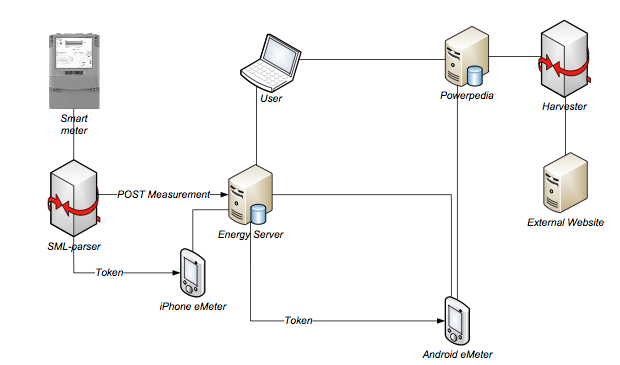
\includegraphics[width=15cm]{Images/emeter_overview.png}
 \label{emeter_overview}
 \caption{Overview over the complete system}
\end{figure}
\end{center}
\todo{replace figure}
Figure~\ref{emeter_overview} depicts a complete overview of the current status of the system. In the original implementation of the eMeter system, there were only the smart meter, SML-parser, Energy Server, User, and iPhone eMeter components. In several refinement steps, the system evolved into what is described hereafter. 

The eMeter gateway polls the smart meter to get the current electricity consumption value and stores it in a database. It also broadcasts the unique identifier (token) of the smart meter, which can be picked up by the iPhone eMeter client to add the corresponding smart meter to the list of accessible smart meters. For the Android application, this token can be found on the eMeter gateway. Both mobile phone applications communicate with the eMeter gateway to get measurement data. The Android version also interacts with PowerPedia. PowerPedia uses the harvester module for data initialization, which gets the corresponding data from external websites. 
PowerPedia and the Energy Server both have a web interface that is accessible by users.    

\subsection{eMeter System}
The eMeter system is an interactive energy consumption monitoring system. It allows users to track the energy usage on a household and device level. By providing instantaneous feedback on the overall energy usage and letting user interactively measure and compare the consumption of individual devices, the system helps to identify where energy is wasted and decrease the overall energy consumption.  

eMeter combines smart electricity meters with a mobile phone application, which makes the system very easy to use.  All the user has to do is downloading the application for the mobile phone over the internet.

The system was first designed and implemented in a bachelor thesis~\cite{roediger}. 

\subsubsection{eMeter Architecture}\label{sec:emeter_architecture}
\missingfigure{eMeter architecture}
The eMeter extends the functionality of the smart electricity meter and consists of multiple decoupled components with different functionalities. Apart from the smart meter, the infrastructure contains the eMeter gateway, which communicates directly with the meter and makes the electricity consumption data available using URLs. Several portable user interfaces allow users to get real-time feedback from the gateway and let users measure and display current consumption data. The communication between the different components is realized over http, in compliance with the "Web of Things" paradigm\cite{guinardWoT:inbook:2010}. This allows a seamless integration of physical resources, such as smart meters or electricity consumption measurements, into the web\cite{recognize_home_appliances}. 

\minisec{Smart electricity meter}
The system builds upon \textit{smart electricity meters}\footnote{e.g Landis+Gyr ZMK410 smart meter, as used in the system}, which allow to monitor the total energy consumption that results from devices attached to the electric circuit of the household in real or near-real time. The meter logs this data in regular intervals. Also, compared to regular meters, smart meters have a communication interface intended for remote reading for billing purposes. There is quite a number of households with smart electricity meters already and this number will be increasing even more\footnote{For example, energy monitoring systems are required for newly build or renovated houses in Europe by law\cite{eu_emeter}}. No further setup or installation is required.

Smart meters used in the eMeter project can be accessed via ethernet. Data can be requested using the SML protocol\footnote{Smart Message Language protocol (SML). The SML specification of the SyM$^2$ can be found here: \url{http://www.vde.com/de/fnn/extras/Sym2/Infomaterial/Documents/SML_081112_103.pd}} 

\minisec{eMeter gateway}
The eMeter gateway is responsible for acquiring and storing data from the smart meter and also for handing requests from the user interface.  
Prior to~\cite{embedded_gateway}, the functionality provided by the eMeter gateway was split into two distinct systems, the SML parser and the Energy Server. 
The SML parser was connected to the smart meter via a LAN-cable. Its task was to read the binary encoded messages and then to forward a relevant subset of the data to the Energy Server as a HTTP message, encoded as a JSON string. The Energy Server was the central instance that stored and managed the measurements from the parser. 
%By having a server between the SML parser and the user interface, clients can access the data using the HTTP protocol. The server also has a web user interface. Statistical information such as total measured energy in kWh or smart meters attached to the system, all the measurements received from the parser and other data can be accessed via this interface. 

The current architecture of the eMeter gateway is slightly different. Both the SML parser and Energy Server are now realized as a standalone embedded gateway referred to as \textit{eMeter gateway}.
Because both components are on the same device now, there is no dependency on Internet anymore. The SML parser can write data polled from the meter directly into the database of the energy server, such that there is no need for the intermediate step of sending messages over the Internet. 

The energy server provides access to the measurement through a RESTful API using JASON as the representation format. Clients can thus use HTTP calls instead of having to know the SML protocol, which would be necessary without the energy server. Also, the server is able to process the collected data and thus offers a richer interface than the smart meter does. 

Additionally to the RESTful API, the server also has a web user interface. Users can brows through statistical information such as total measured energy in kWh or smart meters attached to the system, all the measurements received from the parser and other data using a web browser.

\minisec{Mobile Phone Application}
\begin{center}
\begin{figure}
 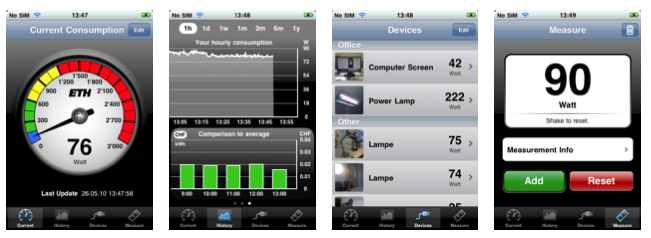
\includegraphics[width=16cm]{Images/iphone_screens.png}
 \label{iphone_screens}
 \caption{Mobile application user interface}
\end{figure}
\end{center}
\todo{Replace image}
In order to motivate users to use the eMeter system over a long-time period, an attractive, easy accessible mobile phone user interface was created. This application is the front-end of the system. It communicates with the Energy Server to aquire electricity usage data.
With this data, the current electricity consumption is visualized in real-time and historical usage is calculated. It also allows users to interactively measure the energy consumption of a single or multiple domestic appliances. 

There are four different views as displayed in figure~\ref{iphone_screens}:

\begin{description}
 \item[Overview] The overview screen shows the current consumption of the household, visualized with the help of a gauge. There are four different colors to help users to classify their current consumption and to compare it to historical consumption. The gauge is self-learning, it adapts the colors and ranges according the consumption. The blue range is the base load.
 \item[History] The history view displays the historic consumption as stored on the Energy Server in a load curve. Statistical information such as cumulative or average, minimum or maximum consumption can be found here as well.
 \item[Measure] In this view, users can interactively measure the consumption or standby usage of a switchable device by clicking on the start button and thereafter turning the device on or off. The result in Watt is displayed right away. The measured device can be stored in the device list of the application that stores all the devices that have been measured. Further information such as picture, location or utilization can be specified.
 \item[Devices] The devices screen shows all the previously created devices. They can be sorted according to their location or energy usage to find the biggest energy guzzlers right away.   
\end{description}
Originally, the mobile phone application was developed in Objective-C for the iPhone.

\subsection{Measurement data}
\subsubsection{Smart Electricity Meter}
Table~\ref{meter_values} denotes the values that are directly acquired from the smart meter. The meter logs electricity consumption data once per second per electrical phase. The name extensions $L1$, $L2$, and $L3$ denote the phase to which the respective value belongs. 
Each phase is thus measured separately. 

\begin{table}[htdp]
\caption{Measurement data acquired from the smart electricity meter\cite{recognize_home_appliances}}
\begin{center}
\begin{tabular}{|p{3cm}|l|l|l|p{4cm}|}
\hline
Value & Quantity & Type & Unit & Explanation \\
\hline
\hline
smartMeterId & identifier & int & ID & identifies smart meter\\
\hline
created on & timestamp & long & Date & time the meter recorded the measurement\\
\hline 
powerL1, powerL2, powerL3 & $P_1$, $P_2$, $P_3$ & double & Watt & real power on $Lx$\\
\hline
currentNeutral & $I_{neu}$ & double & \multirow{2}{*}{Ampere} & current on the wire which is connected to the neutral point \\
\cline{1-3}\cline{5-5}   
currentL1, currentL2, currentL3 & $I_{eff1}$, $I_{eff2}$, $I_{eff3}$ & double & & current on circuit $Lx$\\
\hline
voltageL1, voltageL2, voltageL3 & $U_{eff1}$, $U_{eff2}$, $U_{eff3}$ & double & Volt & voltage on circuit $Lx$\\ 
\hline
phaseShiftCVL1, phaseShiftCVL2, phaseShiftCVL3 & $\phi_1$, $\phi_2$, $\phi_3$ & double & Degree & phase shift between the current component of the fundamental frequency and the voltage on $Lx$\\
\hline      
\end{tabular}
\end{center}
\label{meter_values}
\end{table}%

With these quantities, further information such as apparent, reactive, and distortion power can be derived. 

\subsubsection{Mobile phone client}
When a device is measured on one of the mobile phone clients, a recognition with values as shown in table~\ref{recognition} is created. For both the start and end date of the measurement, the number of watt recorded by the smart meter are determined. To do so, the system uses the algorithm described in~\cite{weiss:inprocPUC:2012}. \todo{which values are used? powerLx? What else would be helpful to record (e.g apparent/reactive/distortion power? Can they be determined?)? }

\begin{table}[htdp]
\caption{Recognition}
\begin{center}
\begin{tabular}{|c|c|p{5cm}|}
\hline
Value & Type & Explanation\\
\hline
\hline
id & ID & unique identifier of recognition \\
deviceId & ID & id of measured device \\ 
startDate & timestamp & time measurement started \\
endDate & timestamp & time measurement ended\\
startWatts & Watt & total energy consumption at starDate  \\
endWatts & Watt & total energy consumption at endDate \\
createdOn & timestamp & time recognition was created\\
userId & ID & id of user recognition is associated to \\
\end{tabular}
\end{center}
\label{recognition}
\end{table}%


\subsection{PowerPedia Prototype}
The PowerPedia prototype is a web platform which serves as a central server for consumption measurement data created by users with the eMeter system. The prototype was build as an independent module of the eMeter system to enhance its features, namely putting electricity consumption values in a larger context beyond mere numbers.

PowerPedia was developed as a means to make the energy consumption more transparent for users~\cite{merklepp}. The main objective of the system was to "allow users to better access their electricity consumption and energy efficiency of their appliances"~\cite{weiss:inprocPUC:2012}. To achieve this goal, the PowerPedia prototype is centered around the idea of action guided feedback. It offers the possibility to compare the energy consumption of household appliances to the consumption of devices that reside in the same device category~\cite{merklepp}. User can upload their measurements made with the eMeter system and get immediate feedback. To help users conserve energy, PowerPedia also provides specific tips on how to be more energy efficient.

\subsubsection{Android eMeter Client}
In order to demonstrate the functionality of PowerPedia, a second version of the mobile phone application was developed. This application was realized as an Android application and is based on the one for the iPhone (as described in~\ref{sec:emeter_architecture}). Is used as a user interface to access the platform.

A detailed analysis of the functionality and technical realization of both the web platform and mobile phone application follows in~\ref{sec:prototype_analysis}.